\PassOptionsToPackage{unicode=true}{hyperref} % options for packages loaded elsewhere
\PassOptionsToPackage{hyphens}{url}
%
\documentclass[]{book}
\usepackage{lmodern}
\usepackage{amssymb,amsmath}
\usepackage{ifxetex,ifluatex}
\usepackage{fixltx2e} % provides \textsubscript
\ifnum 0\ifxetex 1\fi\ifluatex 1\fi=0 % if pdftex
  \usepackage[T1]{fontenc}
  \usepackage[utf8]{inputenc}
  \usepackage{textcomp} % provides euro and other symbols
\else % if luatex or xelatex
  \usepackage{unicode-math}
  \defaultfontfeatures{Ligatures=TeX,Scale=MatchLowercase}
\fi
% use upquote if available, for straight quotes in verbatim environments
\IfFileExists{upquote.sty}{\usepackage{upquote}}{}
% use microtype if available
\IfFileExists{microtype.sty}{%
\usepackage[]{microtype}
\UseMicrotypeSet[protrusion]{basicmath} % disable protrusion for tt fonts
}{}
\IfFileExists{parskip.sty}{%
\usepackage{parskip}
}{% else
\setlength{\parindent}{0pt}
\setlength{\parskip}{6pt plus 2pt minus 1pt}
}
\usepackage{hyperref}
\hypersetup{
            pdftitle={Datenanalyse mit R},
            pdfauthor={Christina Bogner},
            pdfborder={0 0 0},
            breaklinks=true}
\urlstyle{same}  % don't use monospace font for urls
\usepackage{color}
\usepackage{fancyvrb}
\newcommand{\VerbBar}{|}
\newcommand{\VERB}{\Verb[commandchars=\\\{\}]}
\DefineVerbatimEnvironment{Highlighting}{Verbatim}{commandchars=\\\{\}}
% Add ',fontsize=\small' for more characters per line
\usepackage{framed}
\definecolor{shadecolor}{RGB}{248,248,248}
\newenvironment{Shaded}{\begin{snugshade}}{\end{snugshade}}
\newcommand{\AlertTok}[1]{\textcolor[rgb]{0.94,0.16,0.16}{#1}}
\newcommand{\AnnotationTok}[1]{\textcolor[rgb]{0.56,0.35,0.01}{\textbf{\textit{#1}}}}
\newcommand{\AttributeTok}[1]{\textcolor[rgb]{0.77,0.63,0.00}{#1}}
\newcommand{\BaseNTok}[1]{\textcolor[rgb]{0.00,0.00,0.81}{#1}}
\newcommand{\BuiltInTok}[1]{#1}
\newcommand{\CharTok}[1]{\textcolor[rgb]{0.31,0.60,0.02}{#1}}
\newcommand{\CommentTok}[1]{\textcolor[rgb]{0.56,0.35,0.01}{\textit{#1}}}
\newcommand{\CommentVarTok}[1]{\textcolor[rgb]{0.56,0.35,0.01}{\textbf{\textit{#1}}}}
\newcommand{\ConstantTok}[1]{\textcolor[rgb]{0.00,0.00,0.00}{#1}}
\newcommand{\ControlFlowTok}[1]{\textcolor[rgb]{0.13,0.29,0.53}{\textbf{#1}}}
\newcommand{\DataTypeTok}[1]{\textcolor[rgb]{0.13,0.29,0.53}{#1}}
\newcommand{\DecValTok}[1]{\textcolor[rgb]{0.00,0.00,0.81}{#1}}
\newcommand{\DocumentationTok}[1]{\textcolor[rgb]{0.56,0.35,0.01}{\textbf{\textit{#1}}}}
\newcommand{\ErrorTok}[1]{\textcolor[rgb]{0.64,0.00,0.00}{\textbf{#1}}}
\newcommand{\ExtensionTok}[1]{#1}
\newcommand{\FloatTok}[1]{\textcolor[rgb]{0.00,0.00,0.81}{#1}}
\newcommand{\FunctionTok}[1]{\textcolor[rgb]{0.00,0.00,0.00}{#1}}
\newcommand{\ImportTok}[1]{#1}
\newcommand{\InformationTok}[1]{\textcolor[rgb]{0.56,0.35,0.01}{\textbf{\textit{#1}}}}
\newcommand{\KeywordTok}[1]{\textcolor[rgb]{0.13,0.29,0.53}{\textbf{#1}}}
\newcommand{\NormalTok}[1]{#1}
\newcommand{\OperatorTok}[1]{\textcolor[rgb]{0.81,0.36,0.00}{\textbf{#1}}}
\newcommand{\OtherTok}[1]{\textcolor[rgb]{0.56,0.35,0.01}{#1}}
\newcommand{\PreprocessorTok}[1]{\textcolor[rgb]{0.56,0.35,0.01}{\textit{#1}}}
\newcommand{\RegionMarkerTok}[1]{#1}
\newcommand{\SpecialCharTok}[1]{\textcolor[rgb]{0.00,0.00,0.00}{#1}}
\newcommand{\SpecialStringTok}[1]{\textcolor[rgb]{0.31,0.60,0.02}{#1}}
\newcommand{\StringTok}[1]{\textcolor[rgb]{0.31,0.60,0.02}{#1}}
\newcommand{\VariableTok}[1]{\textcolor[rgb]{0.00,0.00,0.00}{#1}}
\newcommand{\VerbatimStringTok}[1]{\textcolor[rgb]{0.31,0.60,0.02}{#1}}
\newcommand{\WarningTok}[1]{\textcolor[rgb]{0.56,0.35,0.01}{\textbf{\textit{#1}}}}
\usepackage{longtable,booktabs}
% Fix footnotes in tables (requires footnote package)
\IfFileExists{footnote.sty}{\usepackage{footnote}\makesavenoteenv{longtable}}{}
\usepackage{graphicx,grffile}
\makeatletter
\def\maxwidth{\ifdim\Gin@nat@width>\linewidth\linewidth\else\Gin@nat@width\fi}
\def\maxheight{\ifdim\Gin@nat@height>\textheight\textheight\else\Gin@nat@height\fi}
\makeatother
% Scale images if necessary, so that they will not overflow the page
% margins by default, and it is still possible to overwrite the defaults
% using explicit options in \includegraphics[width, height, ...]{}
\setkeys{Gin}{width=\maxwidth,height=\maxheight,keepaspectratio}
\setlength{\emergencystretch}{3em}  % prevent overfull lines
\providecommand{\tightlist}{%
  \setlength{\itemsep}{0pt}\setlength{\parskip}{0pt}}
\setcounter{secnumdepth}{5}
% Redefines (sub)paragraphs to behave more like sections
\ifx\paragraph\undefined\else
\let\oldparagraph\paragraph
\renewcommand{\paragraph}[1]{\oldparagraph{#1}\mbox{}}
\fi
\ifx\subparagraph\undefined\else
\let\oldsubparagraph\subparagraph
\renewcommand{\subparagraph}[1]{\oldsubparagraph{#1}\mbox{}}
\fi

% set default figure placement to htbp
\makeatletter
\def\fps@figure{htbp}
\makeatother

\usepackage{booktabs}
\usepackage{amsthm}
\makeatletter
\def\thm@space@setup{%
  \thm@preskip=8pt plus 2pt minus 4pt
  \thm@postskip=\thm@preskip
}
\makeatother


\usepackage{xcolor}
\usepackage{mdframed}
\setlength{\fboxsep}{.8em}

%\definecolor{shadecolor}{rgb}{0.94, 0.97, 1.0}

\newenvironment{rmdinfo}{
  \definecolor{info}{rgb}{0.94, 0.97, 1.0}  %  	Alice blue
  \color{black}
  \begin{mdframed}[backgroundcolor = info]}
 {\end{mdframed}}

\newenvironment{rmdalert}{
  \definecolor{alert}{rgb}{0.96, 0.76, 0.76}  % babypink
  \color{black}
  \begin{mdframed}[backgroundcolor = alert]}
 {\end{mdframed}}


\newenvironment{rmdexample}{
  \definecolor{example}{rgb}{0.0, 0.8, 0.6}  % Caribbean green
  \color{black}
  \begin{mdframed}[backgroundcolor = example]}
 {\end{mdframed}}
 
 
\newenvironment{rmdoutcomes}{
  \definecolor{outcomes}{rgb}{1.0, 0.92, 0.8}  % Blanched Almond
  \color{black}
  \begin{mdframed}[backgroundcolor = outcomes]}
 {\end{mdframed}}

\newenvironment{rmdsummary}{
  \definecolor{summary}{rgb}{1.0, 0.8, 0.5}  % 
  \color{black}
  \begin{mdframed}[backgroundcolor = summary]}
 {\end{mdframed}}
\usepackage{etoolbox}
\makeatletter
\providecommand{\subtitle}[1]{% add subtitle to \maketitle
  \apptocmd{\@title}{\par {\large #1 \par}}{}{}
}
\makeatother
\usepackage[]{natbib}
\bibliographystyle{apalike}

\title{Datenanalyse mit R}
\providecommand{\subtitle}[1]{}
\subtitle{SoSe 2020}
\author{Christina Bogner}
\date{Version vom 24. April 2020}

\begin{document}
\maketitle

{
\setcounter{tocdepth}{1}
\tableofcontents
}
\hypertarget{vorwort}{%
\chapter{Vorwort}\label{vorwort}}

\begin{quote}
``And honey, we're gonna do it in style''
\end{quote}

\hfill --- Fools Garden

\hypertarget{organisatorisches}{%
\section{Organisatorisches}\label{organisatorisches}}

\begin{rmdinfo}
Die Coronaviruspandemie verändert unser Leben und unser Lernen. Die UzK
bittet Lehrende, zumindest zu Beginn des SoSe 2020 auf digitale
Lernformen umzusteigen. Daher wird dieser Kurs als ein Onlinekurs
beginnen. Abhängig von der (sehr dynamischen) Lage werden wir im
weiteren Kursverlauf das Format anpassen. Bitte seien Sie nachsichtig,
wenn nicht alles so klappt, wie in Präsenzveranstaltungen. Wir müssen
aktuell alle sehr viel dazu lernen in Sachen digitale Lehre. Sie können
sicher sein, dass das Geographische Institut bemüht ist, die Lehre so
effizient wie möglich weiter laufen zu lassen, damit Sie in Ihrem
Studium fortfahren können.
\end{rmdinfo}

In dieser Veranstaltung werden wir folgende Werkzeuge verwenden:

\begin{enumerate}
\def\labelenumi{\arabic{enumi}.}
\tightlist
\item
  \textbf{ILIAS}: die Online-Lernplattform der UzK. Entweder sind Sie bereits automatisch in dem Kurs registriert oder werden von mir per Hand angemeldet.
\item
  \textbf{Campuswire}: die Live-Chatplattform dient der allgemeinen Kommunikation und der Selbstorganisation des Lernens. Verwenden Sie diese, um Fragen mit Ihren Kommilitonen und mir zu diskutieren. Sie sollten eine Einladungsmail zu Campuswire erhalten haben.
\item
  \textbf{Zoom}: die Videokonferenz-Software werden wir für live Einführungen nutzen. Die Anmeldemodalitäten sind auf den Kursseiten in ILIAS erklärt.
\end{enumerate}

\hypertarget{sinn-und-unsinn-dieses-skripts}{%
\section{Sinn und Unsinn dieses Skripts}\label{sinn-und-unsinn-dieses-skripts}}

Dieses Skript ist ein lebendiges Begleitdokument des Kurses. Es wird laufend angepasst und aktualisiert.

Ich nutze verschiedene Farbkästen, um wichtige Stellen hervorzuheben:

\begin{rmdinfo}
Infoblock
\end{rmdinfo}

\begin{rmdalert}
Achtung, wichtig!
\end{rmdalert}

\begin{rmdexample}
Beispielblock
\end{rmdexample}

\begin{rmdoutcomes}
Lernziele
\end{rmdoutcomes}

\begin{rmdsummary}
Zusammenfassung
\end{rmdsummary}

\hypertarget{einfuehrung}{%
\chapter{Der Kurs}\label{einfuehrung}}

\hypertarget{zuordnung-zum-modul-und-leistungsnachweis}{%
\section{Zuordnung zum Modul und Leistungsnachweis}\label{zuordnung-zum-modul-und-leistungsnachweis}}

Dieser Kurs gehört zum Modul \emph{Fachmethodik I} oder \emph{Fachmethodik II} und ist aus 4 SWS Praktikum und 2 SWS Seminar aufgebaut. Das wichtigste Ziel besteht darin, Ihnen einen sicheren Umgang mit \texttt{R} beizubringen.

Den Leistungsnachweis bildet ein benoteter Praktikumsbericht.

\hypertarget{lernziele-des-kurses}{%
\section{Lernziele des Kurses}\label{lernziele-des-kurses}}

\begin{rmdoutcomes}
\begin{itemize}
\tightlist
\item
  Daten für Analysen vorbereiten
\item
  eigene wiederverwendbare Skripte schreiben
\item
  eigene Funktionen schreiben
\item
  einfache Datenanalysen durchführen
\item
  Daten visualisieren
\item
  Ergebnisse reproduzierbar im Praktikumsbericht darstellen
\end{itemize}
\end{rmdoutcomes}

\hypertarget{was-mir-im-umgang-miteinander-wichtig-ist}{%
\section{Was mir im Umgang miteinander wichtig ist}\label{was-mir-im-umgang-miteinander-wichtig-ist}}

\begin{itemize}
\tightlist
\item
  Pünktlichkeit bei live und Präsenzsitzungen
\item
  Gute Vorbereitung durch erledigen der blenden learning Einheiten und Hausaufgaben
\item
  Respektieren anderer Meinungen
\item
  Offenheit gegenüber neuen Sichtweisen, Themen und Methoden
\item
  Geduld mit sich selbst und den anderen 😄
\end{itemize}

\hypertarget{erste_schritte}{%
\chapter{Erste Schritte in }\label{erste_schritte}}

\begin{rmdoutcomes}
\begin{itemize}
\tightlist
\item
  Layout und Bedeutung einzelner Fenster in RStudio kennen
\item
  Anweisungen aus dem Skript an die Konsole schicken
\item
  R als Taschenrechner benutzen
\item
  erste Funktionen aufrufen
\item
  Objekte mit eckigen Klammern {[} {]} ansprechen
\item
  R-Hilfeseiten aufrufen
\end{itemize}
\end{rmdoutcomes}

\hypertarget{was-ist-r}{%
\section{Was ist R?}\label{was-ist-r}}

R ist eine Programmiersprache für Datenanalyse und statistische Modellierung. Es ist frei verfügbar (\emph{open source software}) und neben Python einer der am meisten benutzten Programmiersprachen zur Datenanalyse und -visualisierung. R wurde von Ross Ihaka und Robert Gentleman 1996 veröffentlicht \citet{Ihaka1996}. Es gibt für R eine Vielzahl von Zusatzpaketen, die die Funktionalität und die Einsatzmöglichkeiten enorm erweitern.

Sie können R für Ihren Computer auf der offiziellen R-Seite \url{https://www.r-project.org/} herunter laden und installieren. Auch die Pakete finden Sie dort unter CRAN (\emph{The Comprehensive R Archive Network}). Auf den CRAN-Seiten finden Sie sogen. \href{http://cran.r-project.org/web/views/}{CRAN Task Views}, eine Übersicht über Pakete in verschiedenen Themenbereichen. Für den Umweltbereich sind folgende Paketsammlungen besonders relevant:

\begin{itemize}
\tightlist
\item
  Environmetrics: Analyse von Umweltdaten
\item
  Multivariate: Multivariate Statistik
\item
  Spatial: Analyse von räumlichen Daten
\item
  TimeSeries: Zeitreihenanalyse
\end{itemize}

Zu Beginn des Kurses, werden wir jedoch nicht auf Ihren lokalen Rechnern arbeiten, sondern in einer Cloud (s.u.). Das ermöglicht einen schnelleren Einstieg in R und bietet eine live Unterstützung durch den Dozenten beim Programmieren. Daher biete ich zu diesem frühen Zeitpunkt im Kurs keine Unterstützung bei der Installation. Für die ganz Ungeduldigen, gibt es hier eine kurze \emph{Einleitung zur Installation}

\hypertarget{was-ist-rstudio}{%
\section{Was ist RStudio?}\label{was-ist-rstudio}}

RStudio Desktop ist eine Entwicklungsumgebung für R. Sie können die \emph{open source} Version kostenlos für Ihren Rechner \href{https://rstudio.com/products/rstudio/\#rstudio-desktop}{hier} herunterladen.

Es gibt eine live Einführung in RStudio im Kurs. Zusätzlich können Sie hier ein Video dazu ansehen.

\hypertarget{rstudio-cloud}{%
\section{RStudio Cloud}\label{rstudio-cloud}}

Zu Beginn des Kurses werden wir in der \href{https://rstudio.cloud/}{RStudio Cloud} arbeiten. Sie sollten eine Einladungsmail zu unserem Kurs in der Cloud bekommen haben. Ich werde in der Cloud Projekte für Sie anlegen (\emph{assignment}), die Skripte, Arbeitsanweisungen etc. beinhalten. Wenn Sie auf so ein Assignment klicken, wird für Sie automatische ein Kopie des Projekts erstellt, in der Sie dann arbeiten können.

Der große Vorteil der Cloud ist, dass ich direkt in Ihre Projekte eingreifen kann, wenn es mal zu Fehlern kommt. Während ich in Ihrem Projekt arbeite, werden Sie kurz aus der R-Sitzung ausgeloggt, da die Cloud kein gleichzeitiges Arbeiten unterstützt. Nehmen Sie sich etwas Zeit, um die Cloud und die darin enthaltenen \href{https://rstudio.cloud/learn/primers}{Tutorials} kennen zu lernen.

Sowohl in der RStudio Cloud als auch in einer lokalen Installation, ist Ihr RStudio so aufgebaut wie in Abbildung \ref{fig:rstudio}.

\begin{figure}
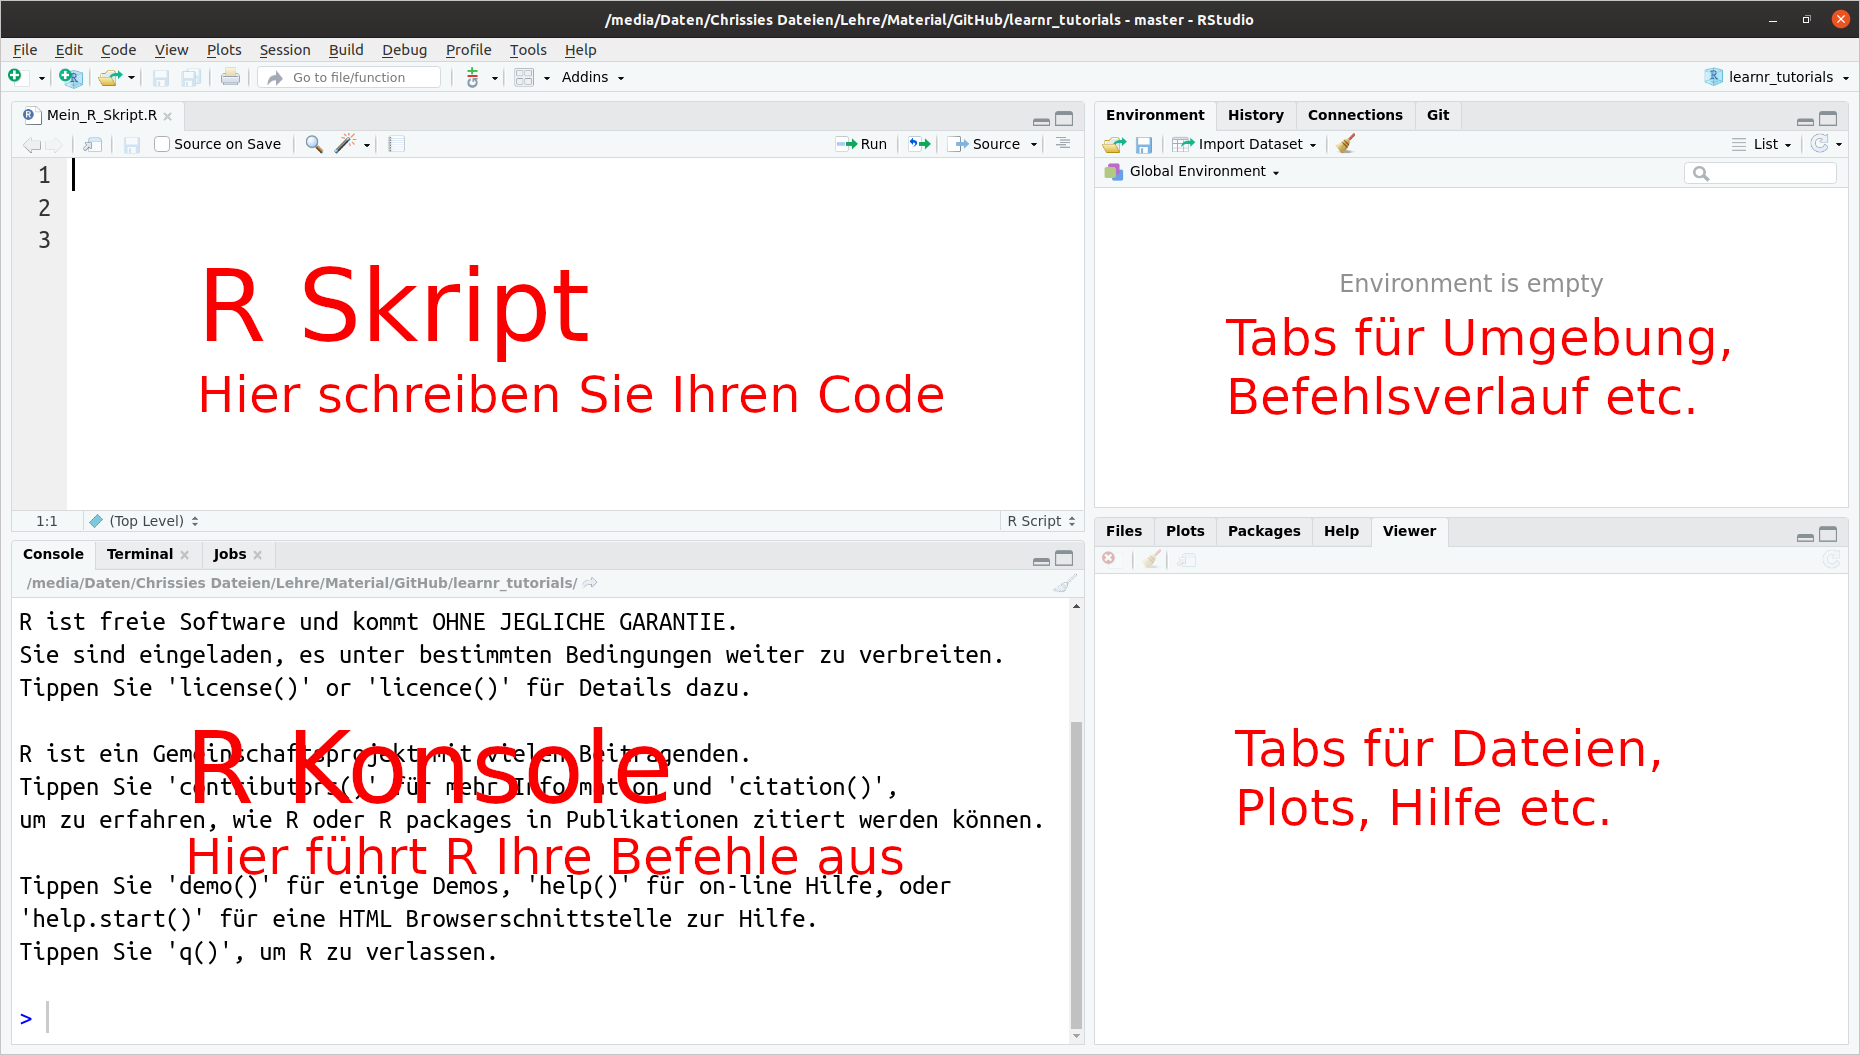
\includegraphics[width=1\linewidth]{RStudio} \caption{Aufbau von RStudio}\label{fig:rstudio}
\end{figure}

\hypertarget{inhalt-der-live-einfuxfchrung-und-der-uxfcbungen}{%
\section{Inhalt der live Einführung und der Übungen}\label{inhalt-der-live-einfuxfchrung-und-der-uxfcbungen}}

\begin{itemize}
\tightlist
\item
  Überblick über RStudio
\item
  R als Taschenrechner
\item
  einfache Funktionen aufrufen
\item
  Zuordnungen (\emph{assignments})
\item
  Notation mit eckigen Klammern {[} {]} (\emph{array}-Notation)
\item
  Hilfeseiten aufrufen
\end{itemize}

Funktionen, die wir in der Session nutzen werden:

\begin{longtable}[]{@{}lll@{}}
\toprule
\begin{minipage}[b]{0.30\columnwidth}\raggedright
Funktion\strut
\end{minipage} & \begin{minipage}[b]{0.28\columnwidth}\raggedright
Bedeutung\strut
\end{minipage} & \begin{minipage}[b]{0.33\columnwidth}\raggedright
Beispielaufruf\strut
\end{minipage}\tabularnewline
\midrule
\endhead
\begin{minipage}[t]{0.30\columnwidth}\raggedright
\texttt{pi}\strut
\end{minipage} & \begin{minipage}[t]{0.28\columnwidth}\raggedright
Zahl pi\strut
\end{minipage} & \begin{minipage}[t]{0.33\columnwidth}\raggedright
\texttt{pi}\strut
\end{minipage}\tabularnewline
\begin{minipage}[t]{0.30\columnwidth}\raggedright
\texttt{sin}\strut
\end{minipage} & \begin{minipage}[t]{0.28\columnwidth}\raggedright
Sinus\strut
\end{minipage} & \begin{minipage}[t]{0.33\columnwidth}\raggedright
\texttt{sin(2)}\strut
\end{minipage}\tabularnewline
\begin{minipage}[t]{0.30\columnwidth}\raggedright
\texttt{cos}\strut
\end{minipage} & \begin{minipage}[t]{0.28\columnwidth}\raggedright
Cosinus\strut
\end{minipage} & \begin{minipage}[t]{0.33\columnwidth}\raggedright
\texttt{cos(2)}\strut
\end{minipage}\tabularnewline
\begin{minipage}[t]{0.30\columnwidth}\raggedright
\texttt{sqrt}\strut
\end{minipage} & \begin{minipage}[t]{0.28\columnwidth}\raggedright
Quadratwurzel\strut
\end{minipage} & \begin{minipage}[t]{0.33\columnwidth}\raggedright
\texttt{sqrt(2)}\strut
\end{minipage}\tabularnewline
\begin{minipage}[t]{0.30\columnwidth}\raggedright
\texttt{c}\strut
\end{minipage} & \begin{minipage}[t]{0.28\columnwidth}\raggedright
(\emph{concatenate}) Fügt Daten zu einem Vektor zusammen\strut
\end{minipage} & \begin{minipage}[t]{0.33\columnwidth}\raggedright
\texttt{c(1,2,3,4)}\strut
\end{minipage}\tabularnewline
\begin{minipage}[t]{0.30\columnwidth}\raggedright
\texttt{help.start}\strut
\end{minipage} & \begin{minipage}[t]{0.28\columnwidth}\raggedright
Öffnet ein Browser-Fenster mit diversen Handbüchern\strut
\end{minipage} & \begin{minipage}[t]{0.33\columnwidth}\raggedright
\texttt{help.start()}\strut
\end{minipage}\tabularnewline
\begin{minipage}[t]{0.30\columnwidth}\raggedright
\texttt{help.search}\strut
\end{minipage} & \begin{minipage}[t]{0.28\columnwidth}\raggedright
Sucht nach einem Begriff in Hilfe-Dateien\strut
\end{minipage} & \begin{minipage}[t]{0.33\columnwidth}\raggedright
\texttt{help.search(\textquotesingle{}time\textquotesingle{})}\strut
\end{minipage}\tabularnewline
\begin{minipage}[t]{0.30\columnwidth}\raggedright
\texttt{??}\strut
\end{minipage} & \begin{minipage}[t]{0.28\columnwidth}\raggedright
alias \texttt{help.search}\strut
\end{minipage} & \begin{minipage}[t]{0.33\columnwidth}\raggedright
\texttt{??time}\strut
\end{minipage}\tabularnewline
\begin{minipage}[t]{0.30\columnwidth}\raggedright
\texttt{help}\strut
\end{minipage} & \begin{minipage}[t]{0.28\columnwidth}\raggedright
Sucht nach einer Funktion\strut
\end{minipage} & \begin{minipage}[t]{0.33\columnwidth}\raggedright
\texttt{?mean}\strut
\end{minipage}\tabularnewline
\begin{minipage}[t]{0.30\columnwidth}\raggedright
\texttt{?}\strut
\end{minipage} & \begin{minipage}[t]{0.28\columnwidth}\raggedright
alias \texttt{help()}\strut
\end{minipage} & \begin{minipage}[t]{0.33\columnwidth}\raggedright
\texttt{?mean}\strut
\end{minipage}\tabularnewline
\begin{minipage}[t]{0.30\columnwidth}\raggedright
\texttt{mean}\strut
\end{minipage} & \begin{minipage}[t]{0.28\columnwidth}\raggedright
Mittelwert\strut
\end{minipage} & \begin{minipage}[t]{0.33\columnwidth}\raggedright
\texttt{mean(c(1,2,3,4))}\strut
\end{minipage}\tabularnewline
\begin{minipage}[t]{0.30\columnwidth}\raggedright
\texttt{var}\strut
\end{minipage} & \begin{minipage}[t]{0.28\columnwidth}\raggedright
Varianz\strut
\end{minipage} & \begin{minipage}[t]{0.33\columnwidth}\raggedright
\texttt{var(c(1,2,3,4))}\strut
\end{minipage}\tabularnewline
\begin{minipage}[t]{0.30\columnwidth}\raggedright
\texttt{sd}\strut
\end{minipage} & \begin{minipage}[t]{0.28\columnwidth}\raggedright
Standardabweichung\strut
\end{minipage} & \begin{minipage}[t]{0.33\columnwidth}\raggedright
\texttt{sd(c(1,2,3,4))}\strut
\end{minipage}\tabularnewline
\begin{minipage}[t]{0.30\columnwidth}\raggedright
\texttt{sum}\strut
\end{minipage} & \begin{minipage}[t]{0.28\columnwidth}\raggedright
Summe\strut
\end{minipage} & \begin{minipage}[t]{0.33\columnwidth}\raggedright
\texttt{sum(c(1,2,3,4))}\strut
\end{minipage}\tabularnewline
\begin{minipage}[t]{0.30\columnwidth}\raggedright
\texttt{vector}\strut
\end{minipage} & \begin{minipage}[t]{0.28\columnwidth}\raggedright
Generiert einen Vektor\strut
\end{minipage} & \begin{minipage}[t]{0.33\columnwidth}\raggedright
\texttt{vector(length=3,\ mode=\textquotesingle{}numeric\textquotesingle{})}\strut
\end{minipage}\tabularnewline
\bottomrule
\end{longtable}

\hypertarget{daten}{%
\chapter{Daten in R}\label{daten}}

\begin{rmdoutcomes}
\begin{itemize}
\tightlist
\item
  Daten einlesen mit \texttt{read.table}
\item
  Datenstrukturen erstellen
\item
  Typen von Daten in R abfragen
\item
  Daten speichern mit \texttt{write.table}
\end{itemize}
\end{rmdoutcomes}

\hypertarget{datenstrukturen-erzeugen}{%
\section{Datenstrukturen erzeugen}\label{datenstrukturen-erzeugen}}

In R gibt es unterschiedliche Datenobjekte. Es ist wichtig, sich über die Struktur (oder Typ) des Datenobjekts Gedanken zu machen. Denn diese bestimmt, was mit einem Objekt gemacht werden kann und ob Funktionen damit richtig umgehen können. Schließlich ist es nicht egal, ob es sich bei einem Objekt um ein numerisches Objekt oder einfach Text (\emph{character}) handelt.

Die wichtigsten Datentypen sind

\begin{itemize}
\tightlist
\item
  \textbf{Vektoren}: hier gruppiert man gleichartige Elemente, z.B. Zahlen. Auch eine einzelne Zahl (ein Skalar) wird von R wie ein Vektor behandelt.
\item
  \textbf{Matrizen}: zweidimensionale (Zeilen und Spalten) Datentabellen mit gleichartigen Elementen.
\item
  \textbf{Listen}: können beliebige Elemente beliebiger Länge enthalten.
\item
  \textbf{Dataframes}: zweidimensionale Datentabellen, die beliebige Elemente enthalten können. Die Spalten der Dataframes müssen allerdings gleichartige Elemente enthalten. Dataframes sind eine Unterart von Listen.
\end{itemize}

Neben diesen Hauptstrukturen gibt es

\begin{itemize}
\tightlist
\item
  \textbf{Factor}: ein besonderer Vektor für kategorielle Variablen
\end{itemize}

Um diese Datenstrukturen zu erzeugen, gibt es jeweils eine Funktion mit gleichlautendem Namen.

\begin{Shaded}
\begin{Highlighting}[]
\CommentTok{# Vektor erzeugen}
\NormalTok{my_vect =}\StringTok{ }\KeywordTok{vector}\NormalTok{(}\DataTypeTok{length =} \DecValTok{3}\NormalTok{, }\DataTypeTok{mode =} \StringTok{'numeric'}\NormalTok{)}
\NormalTok{my_vect}
\end{Highlighting}
\end{Shaded}

\begin{verbatim}
## [1] 0 0 0
\end{verbatim}

\begin{Shaded}
\begin{Highlighting}[]
\CommentTok{# Matrix erzeugen}
\NormalTok{my_matrix =}\StringTok{ }\KeywordTok{matrix}\NormalTok{(}\DataTypeTok{data =} \KeywordTok{c}\NormalTok{(}\DecValTok{1}\OperatorTok{:}\NormalTok{(}\DecValTok{3}\OperatorTok{*}\DecValTok{4}\NormalTok{)), }\DataTypeTok{nrow =} \DecValTok{3}\NormalTok{, }\DataTypeTok{ncol =} \DecValTok{4}\NormalTok{)}
\NormalTok{my_matrix}
\end{Highlighting}
\end{Shaded}

\begin{verbatim}
##      [,1] [,2] [,3] [,4]
## [1,]    1    4    7   10
## [2,]    2    5    8   11
## [3,]    3    6    9   12
\end{verbatim}

\begin{Shaded}
\begin{Highlighting}[]
\CommentTok{# Dataframe erzeugen}
\NormalTok{my_dataframe =}\StringTok{ }\KeywordTok{data.frame}\NormalTok{(}\StringTok{'Spalte_1'}\NormalTok{ =}\StringTok{ }\KeywordTok{rep}\NormalTok{(}\StringTok{'Text'}\NormalTok{, }\DecValTok{10}\NormalTok{),}
                          \StringTok{'Spalte_2'}\NormalTok{ =}\StringTok{ }\DecValTok{1}\OperatorTok{:}\DecValTok{10}\NormalTok{)}
\NormalTok{my_dataframe}
\end{Highlighting}
\end{Shaded}

\begin{verbatim}
##    Spalte_1 Spalte_2
## 1      Text        1
## 2      Text        2
## 3      Text        3
## 4      Text        4
## 5      Text        5
## 6      Text        6
## 7      Text        7
## 8      Text        8
## 9      Text        9
## 10     Text       10
\end{verbatim}

\begin{Shaded}
\begin{Highlighting}[]
\CommentTok{# Liste erzeugen}
\NormalTok{my_list =}\StringTok{ }\KeywordTok{list}\NormalTok{(}\StringTok{'Schachtel_1'}\NormalTok{ =}\StringTok{ }\DecValTok{3}\NormalTok{, }\StringTok{'Schachtel_2'}\NormalTok{ =}\StringTok{ }\NormalTok{my_dataframe,}
               \StringTok{'Schachtel_3'}\NormalTok{ =}\StringTok{ 'Noch mehr Text'}\NormalTok{)}
\NormalTok{my_list}
\end{Highlighting}
\end{Shaded}

\begin{verbatim}
## $Schachtel_1
## [1] 3
## 
## $Schachtel_2
##    Spalte_1 Spalte_2
## 1      Text        1
## 2      Text        2
## 3      Text        3
## 4      Text        4
## 5      Text        5
## 6      Text        6
## 7      Text        7
## 8      Text        8
## 9      Text        9
## 10     Text       10
## 
## $Schachtel_3
## [1] "Noch mehr Text"
\end{verbatim}

\begin{Shaded}
\begin{Highlighting}[]
\CommentTok{# Factor erzeugen}
\NormalTok{my_factor =}\StringTok{ }\KeywordTok{factor}\NormalTok{(}\KeywordTok{c}\NormalTok{(}\StringTok{'R'}\NormalTok{, }\StringTok{'RStudio'}\NormalTok{, }\StringTok{'Cloud'}\NormalTok{, }\StringTok{'Cloud'}\NormalTok{, }\StringTok{'R'}\NormalTok{, }\StringTok{'R'}\NormalTok{))}
\NormalTok{my_factor}
\end{Highlighting}
\end{Shaded}

\begin{verbatim}
## [1] R       RStudio Cloud   Cloud   R       R      
## Levels: Cloud R RStudio
\end{verbatim}

\hypertarget{arten-von-daten-in-r}{%
\section{Arten von Daten in R}\label{arten-von-daten-in-r}}

Die Datenstrukturen \texttt{vector}, \texttt{data.frame} usw. können unterschiedliche Arten von Daten enthalten.

\begin{longtable}[]{@{}ll@{}}
\toprule
Name & Beispiele\tabularnewline
\midrule
\endhead
raw & 3A, FE\tabularnewline
logical & TRUE, FALSE\tabularnewline
integer & 1, 42, -3\tabularnewline
numeric/double & 3, 2.81, 6.032e23\tabularnewline
complex & 1.2+2.2i\tabularnewline
character & ``foo''\tabularnewline
\bottomrule
\end{longtable}

\hypertarget{objekt-sag-mir-wer-du-bist}{%
\section{Objekt, sag mir wer du bist}\label{objekt-sag-mir-wer-du-bist}}

Um die Struktur und/oder Datenart abzufragen, verwendet man \texttt{class}, \texttt{typeof}, \texttt{mode} und \texttt{storage.mode}.

\begin{Shaded}
\begin{Highlighting}[]
\KeywordTok{class}\NormalTok{(my_vect)}
\end{Highlighting}
\end{Shaded}

\begin{verbatim}
## [1] "numeric"
\end{verbatim}

\begin{Shaded}
\begin{Highlighting}[]
\KeywordTok{typeof}\NormalTok{(my_vect)}
\end{Highlighting}
\end{Shaded}

\begin{verbatim}
## [1] "double"
\end{verbatim}

\begin{Shaded}
\begin{Highlighting}[]
\KeywordTok{class}\NormalTok{(my_dataframe)}
\end{Highlighting}
\end{Shaded}

\begin{verbatim}
## [1] "data.frame"
\end{verbatim}

\begin{Shaded}
\begin{Highlighting}[]
\KeywordTok{typeof}\NormalTok{(my_dataframe)}
\end{Highlighting}
\end{Shaded}

\begin{verbatim}
## [1] "list"
\end{verbatim}

Mit \texttt{str} kann man das Innenleben eines Objekts anzeigen. Das ist besonders wichtig nach dem Einlesen von Daten, um das Ergebnis des Einlesens zu kontrollieren. Dabei kontrolliert man, dass z.B. alle numerischen Spalten auch als Zahlen eingelesen wurden und nichts schief gegangen ist.

\begin{Shaded}
\begin{Highlighting}[]
\KeywordTok{str}\NormalTok{(my_dataframe)}
\end{Highlighting}
\end{Shaded}

\begin{verbatim}
## 'data.frame':    10 obs. of  2 variables:
##  $ Spalte_1: Factor w/ 1 level "Text": 1 1 1 1 1 1 1 1 1 1
##  $ Spalte_2: int  1 2 3 4 5 6 7 8 9 10
\end{verbatim}

Weiter Funktionen, die Auskunft über Objekte geben sind \texttt{length}, sinnvoll auf nur Vektoren und Listen, und \texttt{dim}, sinnvoll auf zweidimensionalen Datenobjekten. Wenn Sie versuchen, \texttt{dim} auf einem Vektor aufzurufen, gibt es \texttt{NULL} (s.u.), weil Vektoren keine Dimensionen haben. Wenn Sie \texttt{length} auf einem \texttt{data.frame} aufrufen, bekommen Sie die Anzahl der Dimensionen, nämlich 2. Das sind keine besonders spannenden Informationen 😄.

\begin{Shaded}
\begin{Highlighting}[]
\KeywordTok{length}\NormalTok{(my_vect)}
\end{Highlighting}
\end{Shaded}

\begin{verbatim}
## [1] 3
\end{verbatim}

\begin{Shaded}
\begin{Highlighting}[]
\KeywordTok{dim}\NormalTok{(my_vect)}
\end{Highlighting}
\end{Shaded}

\begin{verbatim}
## NULL
\end{verbatim}

\begin{Shaded}
\begin{Highlighting}[]
\KeywordTok{length}\NormalTok{(my_dataframe)}
\end{Highlighting}
\end{Shaded}

\begin{verbatim}
## [1] 2
\end{verbatim}

\begin{Shaded}
\begin{Highlighting}[]
\KeywordTok{dim}\NormalTok{(my_dataframe)}
\end{Highlighting}
\end{Shaded}

\begin{verbatim}
## [1] 10  2
\end{verbatim}

\hypertarget{datenluxfccken-fehlschluxe4ge-etc.}{%
\section{Datenlücken, Fehlschläge etc.}\label{datenluxfccken-fehlschluxe4ge-etc.}}

Datenlücken werden in R mit \texttt{NA} kodiert, Fehlschläge bei Berechnungen mit \texttt{NaN} (not a number) und Vektoren der Länge 0 mit \texttt{NULL}. Letzteres wird häufig beim Aufruf von Funktionen benutzt, wenn man bestimmte Parameter ausschalten möchte. Die Benutzung muss aber immer in der Hilfe zur jeweiligen Funktion nachgeschlagen werden.

\hypertarget{inhalt-der-live-einfuxfchrung-und-der-uxfcbungen-1}{%
\section{Inhalt der live Einführung und der Übungen}\label{inhalt-der-live-einfuxfchrung-und-der-uxfcbungen-1}}

\begin{itemize}
\tightlist
\item
  Daten einlesen und \texttt{data.frame} erstellen: Aufgabe \ref{bestandesaufnahme}
\end{itemize}

Funktionen, die wir in der Session nutzen werden:

\begin{longtable}[]{@{}lll@{}}
\toprule
\begin{minipage}[b]{0.30\columnwidth}\raggedright
Funktion\strut
\end{minipage} & \begin{minipage}[b]{0.28\columnwidth}\raggedright
Bedeutung\strut
\end{minipage} & \begin{minipage}[b]{0.33\columnwidth}\raggedright
Beispielaufruf\strut
\end{minipage}\tabularnewline
\midrule
\endhead
\begin{minipage}[t]{0.30\columnwidth}\raggedright
\texttt{read.table}\strut
\end{minipage} & \begin{minipage}[t]{0.28\columnwidth}\raggedright
Liest Daten aus einer Datei ein.\strut
\end{minipage} & \begin{minipage}[t]{0.33\columnwidth}\raggedright
\texttt{read.table(file=\ \textquotesingle{}Daten.txt\textquotesingle{},\ header=TRUE)}\strut
\end{minipage}\tabularnewline
\begin{minipage}[t]{0.30\columnwidth}\raggedright
\texttt{ls}\strut
\end{minipage} & \begin{minipage}[t]{0.28\columnwidth}\raggedright
Zeigt den Inhalt des Workspaces.\strut
\end{minipage} & \begin{minipage}[t]{0.33\columnwidth}\raggedright
\texttt{ls}\strut
\end{minipage}\tabularnewline
\begin{minipage}[t]{0.30\columnwidth}\raggedright
\texttt{head}\strut
\end{minipage} & \begin{minipage}[t]{0.28\columnwidth}\raggedright
Zeigt den ersten Teil eines Objekts.\strut
\end{minipage} & \begin{minipage}[t]{0.33\columnwidth}\raggedright
\texttt{head(x)}\strut
\end{minipage}\tabularnewline
\begin{minipage}[t]{0.30\columnwidth}\raggedright
\texttt{tail}\strut
\end{minipage} & \begin{minipage}[t]{0.28\columnwidth}\raggedright
Zeigt den letzten Teil eines Objekts.\strut
\end{minipage} & \begin{minipage}[t]{0.33\columnwidth}\raggedright
\texttt{tail(x)}\strut
\end{minipage}\tabularnewline
\begin{minipage}[t]{0.30\columnwidth}\raggedright
\texttt{str}\strut
\end{minipage} & \begin{minipage}[t]{0.28\columnwidth}\raggedright
Zeigt die Struktur (Innenleben) eines Objekts an\strut
\end{minipage} & \begin{minipage}[t]{0.33\columnwidth}\raggedright
\texttt{str(my\_dataframe)}\strut
\end{minipage}\tabularnewline
\begin{minipage}[t]{0.30\columnwidth}\raggedright
\texttt{length}\strut
\end{minipage} & \begin{minipage}[t]{0.28\columnwidth}\raggedright
Gibt die Länge eines Objekts.\strut
\end{minipage} & \begin{minipage}[t]{0.33\columnwidth}\raggedright
\texttt{length(x)}\strut
\end{minipage}\tabularnewline
\begin{minipage}[t]{0.30\columnwidth}\raggedright
\texttt{dim}\strut
\end{minipage} & \begin{minipage}[t]{0.28\columnwidth}\raggedright
Gibt die Dimension eines Objekts (Reihenfolge: Zeilen, Spalten)\strut
\end{minipage} & \begin{minipage}[t]{0.33\columnwidth}\raggedright
\texttt{dim(x)}\strut
\end{minipage}\tabularnewline
\begin{minipage}[t]{0.30\columnwidth}\raggedright
\texttt{seq}\strut
\end{minipage} & \begin{minipage}[t]{0.28\columnwidth}\raggedright
Erstellt eine regelmäßige Reihe.\strut
\end{minipage} & \begin{minipage}[t]{0.33\columnwidth}\raggedright
\texttt{seq(from=-2,\ to=4,\ by=0.1)}\strut
\end{minipage}\tabularnewline
\begin{minipage}[t]{0.30\columnwidth}\raggedright
\texttt{data.frame}\strut
\end{minipage} & \begin{minipage}[t]{0.28\columnwidth}\raggedright
Erstellt eine Datentabelle.\strut
\end{minipage} & \begin{minipage}[t]{0.33\columnwidth}\raggedright
\texttt{data.frame(x,y,z)}\strut
\end{minipage}\tabularnewline
\begin{minipage}[t]{0.30\columnwidth}\raggedright
\texttt{colnames}, \texttt{rownames}\strut
\end{minipage} & \begin{minipage}[t]{0.28\columnwidth}\raggedright
Benennt Spalten bzw. Zeilen eines Datenobjekts.\strut
\end{minipage} & \begin{minipage}[t]{0.33\columnwidth}\raggedright
\texttt{colnames(x)}\strut
\end{minipage}\tabularnewline
\begin{minipage}[t]{0.30\columnwidth}\raggedright
\texttt{rm}\strut
\end{minipage} & \begin{minipage}[t]{0.28\columnwidth}\raggedright
Löscht Objekte aus dem Workspace.\strut
\end{minipage} & \begin{minipage}[t]{0.33\columnwidth}\raggedright
\texttt{rm(x)}\strut
\end{minipage}\tabularnewline
\begin{minipage}[t]{0.30\columnwidth}\raggedright
\texttt{summary}\strut
\end{minipage} & \begin{minipage}[t]{0.28\columnwidth}\raggedright
Fasst ein Objekt zusammen.\strut
\end{minipage} & \begin{minipage}[t]{0.33\columnwidth}\raggedright
\texttt{summary(x)}\strut
\end{minipage}\tabularnewline
\begin{minipage}[t]{0.30\columnwidth}\raggedright
\texttt{table}\strut
\end{minipage} & \begin{minipage}[t]{0.28\columnwidth}\raggedright
Erstellt eine Häufigkeitstabelle.\strut
\end{minipage} & \begin{minipage}[t]{0.33\columnwidth}\raggedright
\texttt{table(x)}\strut
\end{minipage}\tabularnewline
\begin{minipage}[t]{0.30\columnwidth}\raggedright
\texttt{which}\strut
\end{minipage} & \begin{minipage}[t]{0.28\columnwidth}\raggedright
Gibt die TRUE-Indices eines logischen Objekts.\strut
\end{minipage} & \begin{minipage}[t]{0.33\columnwidth}\raggedright
\texttt{which(LETTERS\ ==\ \textquotesingle{}R\textquotesingle{})}\strut
\end{minipage}\tabularnewline
\begin{minipage}[t]{0.30\columnwidth}\raggedright
\texttt{history}\strut
\end{minipage} & \begin{minipage}[t]{0.28\columnwidth}\raggedright
Zeigt die Liste mit ausgeführten Befehlen der Session.\strut
\end{minipage} & \begin{minipage}[t]{0.33\columnwidth}\raggedright
\texttt{history}\strut
\end{minipage}\tabularnewline
\begin{minipage}[t]{0.30\columnwidth}\raggedright
\texttt{write.table}\strut
\end{minipage} & \begin{minipage}[t]{0.28\columnwidth}\raggedright
Speichert Datenobjekte als Tabelle ab.\strut
\end{minipage} & \begin{minipage}[t]{0.33\columnwidth}\raggedright
\texttt{write.table(x,\ file=\textquotesingle{}Tabelle.txt\textquotesingle{})}\strut
\end{minipage}\tabularnewline
\begin{minipage}[t]{0.30\columnwidth}\raggedright
\texttt{save.image}\strut
\end{minipage} & \begin{minipage}[t]{0.28\columnwidth}\raggedright
Speichert den Workspace.\strut
\end{minipage} & \begin{minipage}[t]{0.33\columnwidth}\raggedright
\texttt{save.image(file=\ \textquotesingle{}RSession.Rdata\textquotesingle{})}\strut
\end{minipage}\tabularnewline
\begin{minipage}[t]{0.30\columnwidth}\raggedright
\texttt{savehistory}\strut
\end{minipage} & \begin{minipage}[t]{0.28\columnwidth}\raggedright
Speichert die History.\strut
\end{minipage} & \begin{minipage}[t]{0.33\columnwidth}\raggedright
\texttt{savehistory(file=\ \textquotesingle{}Myhistory.Rhistory\textquotesingle{})}\strut
\end{minipage}\tabularnewline
\bottomrule
\end{longtable}

\hypertarget{aufgabensammlung}{%
\chapter{Aufgabensammlung}\label{aufgabensammlung}}

\hypertarget{erste-schritte}{%
\section{Erste Schritte}\label{erste-schritte}}

\hypertarget{ars-haushaltsbuch}{%
\subsection{Ars Haushaltsbuch}\label{ars-haushaltsbuch}}

Der angehende Datenanalyst Ar Stat möchte dem Rat seiner Mutter folgen und ein Haushaltsbuch anlegen. Als erstes möchte er sich einen Überblick über seine Ausgaben in der Uni-Mensa verschaffen und erstellt die folgende Tabelle:

\begin{table}

\caption{\label{tab:unnamed-chunk-19}Ars Mensaausgaben}
\centering
\begin{tabular}[t]{lr}
\toprule
Wochentag & Ausgaben\\
\midrule
Montag & 2,57\\
Dienstag & 2,90\\
Mittwoch & 2,73\\
Donnerstag & 3,23\\
Freitag & 3,90\\
\bottomrule
\end{tabular}
\end{table}

\begin{enumerate}
\def\labelenumi{\arabic{enumi}.}
\tightlist
\item
  Wie viel hat Ar insgesamt in der Woche ausgegeben?
\item
  Wie viel hat er im Schnitt pro Tag ausgegeben?
\item
  Wie stark schwanken seine Ausgaben?
\end{enumerate}

Leider hat Ar sich beim übertragen der Daten vertippt. Er hat am Dienstag seine Freundin zum Essen eingeladen und 7,95 € statt 2,90 € ausgegeben.

\begin{enumerate}
\def\labelenumi{\arabic{enumi}.}
\setcounter{enumi}{3}
\tightlist
\item
  Korrigieren Sie Ars Fehler.
\item
  Wie verändern sich die Ergebnisse aus den Teilaufgaben 1 bis 3 Warum?
\end{enumerate}

\hypertarget{laden-und-speichern-von-daten}{%
\section{Laden und Speichern von Daten}\label{laden-und-speichern-von-daten}}

\hypertarget{bestandesaufnahme}{%
\subsection{Bestandesaufnahme}\label{bestandesaufnahme}}

Ar Stat arbeitet als HiWi in der AG Ökosystemforschung und soll im Nationalpark Eifel eine Bestandsaufnahme durchführen. Er notiert den BHD (Brusthöhendurchmesser) und die Art der Bäume.

\begin{enumerate}
\def\labelenumi{\arabic{enumi}.}
\tightlist
\item
  Lesen Sie den Datensatz \texttt{BHD.txt} ein und ordnen Sie ihn der Variable \texttt{BHD} zu.
\item
  Erstellen Sie einen Vektor \texttt{a} mit Baumnummern. Von welcher Art sind die Elemente des Vektors \texttt{a}?
\item
  Fügen Sie die Datensätze \texttt{BHD} und \texttt{a} zu einem \texttt{data.frame} zusammen und benennen Sie die Spalten sinnvoll.
\item
  Löschen Sie den Vektor \texttt{a}.
\item
  Lesen Sie den Datensatz \texttt{Art.txt} ein und ordnen Sie ihn der Variablen \texttt{art} zu.
\item
  Fügen Sie die Art in den \texttt{data.frame} ein.
\item
  Erstellen Sie eine Tabelle mit der Anzahl der jeweiligen Arten. Nutzen Sie die Funktion `table'.
\item
  Speichern Sie die Tabelle mit \texttt{write.table}.
\item
  Welche Baumart hat im Mittel einen größeren Brusthöhendurchmesser?
\end{enumerate}

\hypertarget{automatisieren-skripte-funktionen}{%
\section{Automatisieren: Skripte \& Funktionen}\label{automatisieren-skripte-funktionen}}

\hypertarget{r-hausaufgaben}{%
\subsection{R-Hausaufgaben}\label{r-hausaufgaben}}

An dem Kurs ``Einführung in R'' nehmen 49 Studierende teil. Der Leistungsnachweis besteht aus Hausaufgaben, die insgesamt mit 100 Punkten bewertet werden. Ab 50 Punkten gilt der Kurs als bestanden.

\begin{enumerate}
\def\labelenumi{\arabic{enumi}.}
\tightlist
\item
  Lesen Sie den Datensatz \texttt{R-HAs.txt}, der die Endpunkte enthält, ein.
\item
  Ermitteln Sie, wie viele Teilnehmer bestanden und wie viele nicht bestanden haben.
\end{enumerate}

\hypertarget{fledermuxe4use-die-zweite}{%
\subsection{Fledermäuse, die Zweite}\label{fledermuxe4use-die-zweite}}

Wir beschäftigen uns erneut mit den Fledermäusen.

\begin{enumerate}
\def\labelenumi{\arabic{enumi}.}
\tightlist
\item
  Lesen Sie den korrigierten(!) Datensatz \textbackslash{}texttt\{Fledermaus\_cor.txt\} ein.
\item
  Schreiben Sie eine Funktion, die den Entwicklungsstand der Tiere klassifiziert. Nutzen Sie dazu die ad hoc Regel: Individuum \textless{} 5 cm ist ein Jungtier, sonst erwachsen.
\item
  Erstellen Sie eine ordinal-skalierte Variable \texttt{alter} mit dem Entwicklungsstand der Tiere.
\item
  Schreiben Sie eine Funktion, die die Mittelwerte der Größe für weibliche und männliche Individuen berechnet.
\item
  Berechnen Sie die Mittelwerte der Größe und runden Sie auf 2 Nachkommastellen.
\end{enumerate}

\hypertarget{unfaire-klausur}{%
\subsection{Unfaire Klausur?}\label{unfaire-klausur}}

Ar belegt im 4. Semester die Veranstaltung ``Spaß mit R''. Bei der Klausur gibt es 2 Aufgabengruppen mit jeweils 60 Punkten. Aufgabengruppe 1 wird an Studierende auf ungeraden Sitzplätzen und Aufgabengruppe 2 an Studierende auf geraden Sitzplätzen ausgegeben.

\begin{enumerate}
\def\labelenumi{\arabic{enumi}.}
\tightlist
\item
  Lesen Sie den Datensatz \texttt{Klausurpunkte.txt} ein.
\item
  Überprüfen Sie Ars Vermutung, dass die Aufgabengruppe 1 im Schnitt leichter war als Aufgabengruppe 2 (d.h. in der Gruppe 1 im Schnitt mehr Punkte erzielt wurden).
\end{enumerate}

\hypertarget{daten-visualisieren}{%
\section{Daten visualisieren}\label{daten-visualisieren}}

\hypertarget{lange-bramke-harz}{%
\subsection{Lange Bramke (Harz)}\label{lange-bramke-harz}}

Im Harz wurden über eine längere Zeit Niederschlag, Abfluss und Temperatur gemessen.

\begin{enumerate}
\def\labelenumi{\arabic{enumi}.}
\tightlist
\item
  Laden Sie den Datensatz \texttt{Data.dat}.
\item
  Stellen Sie die Temperatur in einem Scatterplot dar. Welche Darstellungsart (Argument \texttt{type} in \texttt{plot}) erscheint Ihnen am sinnvollsten?
\item
  Beschriften Sie die Graphik und fügen Sie einen Titel hinzu.
\item
  Speichern Sie die Graphik als pdf ab.
\item
  Stellen Sie die Niederschläge in einem Diagramm dar. Wählen Sie einen geeigneten Darstellungstyp mit \texttt{type} (Tipp: geben Sie für die Hilfe \texttt{?plot} in die Console ein).
\end{enumerate}

\hypertarget{temperatur-datensatz}{%
\subsection{Temperatur-Datensatz}\label{temperatur-datensatz}}

\begin{enumerate}
\def\labelenumi{\arabic{enumi}.}
\tightlist
\item
  Laden Sie den Temperatur-Datensatz aus \citet{Zuur2009a}.
\item
  Berechnen Sie die Monatsmittelwerte für alle Stationen, sowie die Standardabweichungen.
\item
  Stellen Sie die Monatsmittel der Temperatur in einem Barplot dar.
\item
  Beschriften Sie die Graphik sinnvoll.
\item
  Fügen Sie die Standardabweichungen zu den einzelnen Balken hinzu.
\end{enumerate}

\hypertarget{artenvielfalt-in-grasluxe4ndern}{%
\subsection{Artenvielfalt in Grasländern}\label{artenvielfalt-in-grasluxe4ndern}}

Sie erhalten Daten aus dem Grasland-Monitoring im Yellowstone Nationalpark und dem National Bison Range (USA). Das Ziel des Monitorings ist die Untersuchung möglicher Änderungen der Biodiversität und des Zusammenhang mit Umweltfaktoren. Biodiversität wurde durch die Anzahl unterschiedlicher Arten quantifiziert. Insgesamt haben die Forscher ca. 90 Arten in 8 Transekten kartiert. Die Aufnahmen wurden alle 4 bis 10 Jahre wiederholt. Insgesamt liegen 58 Beobachtungen vor. Die Daten sind in der Datei \texttt{Vegetation2.xls} gespeichert.

\begin{enumerate}
\def\labelenumi{\arabic{enumi}.}
\item
  Laden Sie den Datensatz in R und sehen Sie sich das Ergebnis genau mit \texttt{str}, \texttt{head} und \texttt{tail} an. Diese Aufgabe dient dazu, das Einlesen von Excel-Dateien zu erarbeiten. Tipp: eine mögliche Bibliothek, die dabei helfen kann, wäre \texttt{xlsx}.
\item
  Berechnen Sie den Mittelwert und die Standardabweichung der Artenzahl (Variable \texttt{R}) pro Transekt.
\item
  Plotten Sie die Artenzahl gegen die Variable \texttt{BARESOIL} (Anteil von unbewachsenem Boden).
\item
  Benutzen Sie unterschiedliche Symbole pro Transekt, erstellen Sie eine Legende.
\item
  Beschriften Sie die Graphik sinnvoll und speichern Sie sie als pdf ab, ohne die Maus zu benutzen.
\end{enumerate}

\hypertarget{tracerversuche}{%
\subsection{Tracerversuche}\label{tracerversuche}}

Im Waldstein wurden Tracerversuche mit dem Farbstoff Brilliant Blue durchgeführt und die gefärbten Bodenprofile \emph{binärisiert} (d.h. in ein schwarz-weiß Bild umgewandelt). Schwarze Pixels stellen gefärbten Boden und weiße ungefärbten dar. Aus diesen Binärbildern wurde anschließend eine Reihe von Kenngrößen berechnet.

\begin{enumerate}
\def\labelenumi{\arabic{enumi}.}
\tightlist
\item
  Lesen Sie die Datei \textbackslash{}texttt\{Waldstein2005\_ind.txt\} ein. Die Tiefe eines Profils ist 579 Pixel und es liegen 6 Profile untereinander in der Spalte d.
\item
  Berechnen Sie die 5\%, 50\% und 95\% Quantile des Färbeanteils (Index d) der 6 Profile.
\item
  Stellen Sie den Median des Anteils der Färbung mit der Tiefe dar und fügen Sie die Quantile als transparente Fläche hinzu (Tipp: \texttt{polygon}).
\end{enumerate}

\hypertarget{effizientes-programmieren}{%
\section{Effizientes Programmieren}\label{effizientes-programmieren}}

\hypertarget{lagerungsdichten}{%
\subsection{Lagerungsdichten}\label{lagerungsdichten}}

Auf 10 verschiedenen landwirtschaftlichen Feldern wurden im Oberboden je 25 Stechzylinder entnommen.

\begin{enumerate}
\def\labelenumi{\arabic{enumi}.}
\tightlist
\item
  Lesen Sie den Datensatz r file.name(``Bodendaten.txt'')` ein.
\item
  Bestimmen Sie die mittlere Lagerungsdichte pro Feld.
\end{enumerate}

\hypertarget{temperatur-datensatz-revisited}{%
\subsection{Temperatur-Datensatz, revisited}\label{temperatur-datensatz-revisited}}

\begin{enumerate}
\def\labelenumi{\arabic{enumi}.}
\tightlist
\item
  Laden Sie den Temperatur-Datensatz aus \citet{Zuur2009a}, Datei \texttt{Temperatur.csv}.
\item
  Berechnen Sie die Jahresmittelwerte je Station. (Tipp: Hilfe von \texttt{tapply} genau lesen!)
\end{enumerate}

\hypertarget{refs}{}

\bibliography{book.bib,packages.bib}

\end{document}
